%!TEX root = ../quantum.tex
% Тип документа
\documentclass[a4paper,14pt]{extarticle}

% Шрифты, кодировки, символьные таблицы, переносы
\usepackage{cmap}
\usepackage[T2A]{fontenc}
\usepackage[utf8]{inputenc}
\usepackage[russian]{babel}
% Это пакет -- хитрый пакет, он нужен но не нужен
\usepackage[mode=buildnew]{standalone}

\usepackage
	{
		% Дополнения Американского математического общества (AMS)
		amssymb,
		amsfonts,
		amsmath,
		amsthm,
		physics,
		% misccorr,
		% 
		% Графики и рисунки
		wrapfig,
		graphicx,
		subcaption,
		float,
		tikz,
		tikz-3dplot,
		caption,
		csvsimple,
		color,
		booktabs,
		geometry,
		% 
		% Таблицы, списки
		makecell,
		multirow,
		indentfirst,
		%
		% Интегралы и прочие обозначения
		ulem,
		esint,
		esdiff,
		% 
		% Колонтитулы
		fancyhdr,
	}  

\usepackage{xcolor}
\usepackage{hyperref}

 % Цвета для гиперссылок
\definecolor{linkcolor}{HTML}{000000} % цвет ссылок
\definecolor{urlcolor}{HTML}{799B03} % цвет гиперссылок
 
\hypersetup{pdfstartview=FitH,linkcolor=linkcolor,urlcolor=urlcolor, colorlinks=true}
\hypersetup{pageanchor=false}
% Увеличенный межстрочный интервал, французские пробелы
\linespread{1.3} 
\frenchspacing 

 
% \usetikzlibrary
% 	{
% 		decorations.pathreplacing,
% 		decorations.pathmorphing,
% 		patterns,
% 		calc,
% 		scopes,
% 		arrows,
% 		fadings,
% 		through,
% 		shapes.misc,
% 		arrows.meta,
% 		3d,
% 		quotes,
% 		angles,
% 		babel
% 	}
% Среднее <#1>
\newcommand{\mean}[1]{\langle#1\rangle}
\newcommand{\definition}{\underset{def}{=}}
\renewcommand{\big}{\displaystyle}
% \newcommand{\bra}[1]{\langle#1|}
% \newcommand{\ket}[1]{|#1\rangle#1}
% const прямым шрифтом
\newcommand\ct[1]{\text{\rmfamily\upshape #1}}
\newcommand*{\const}{\ct{const}}
\usepackage{array}
\usepackage{pstool}

\geometry		
	{
		left			=	2cm,
		right 			=	2cm,
		top 			=	2.5cm,
		bottom 			=	2.5cm,
		bindingoffset	=	0cm
	}

%%%%%%%%%%%%%%%%%%%%%%%%%%%%%%%%%%%%%%%%%%%%%%%%%%%%%%%%%%%%%%%%%%%%%%%%%%%%%%%
	%применим колонтитул к стилю страницы
\pagestyle{fancy} 
	%очистим "шапку" страницы
% \fancyhead{} 
	%слева сверху на четных и справа на нечетных
\fancyhead[R]{} 
	%справа сверху на четных и слева на нечетных
\fancyhead[L]{Квантовая механика} 
	%очистим "подвал" страницы
% \fancyfoot{} 
	% номер страницы в нижнем колинтуле в центре
\fancyfoot[C]{\thepage} 

%%%%%%%%%%%%%%%%%%%%%%%%%%%%%%%%%%%%%%%%%%%%%%%%%%%%%%%%%%%%%%%%%%%%%%%%%%%%%%%

\renewcommand{\contentsname}{Оглавление}
\usepackage{tocloft}
\usepackage{secdot}
\sectiondot{subsection}
\begin{document}

\tableofcontents
\newpage

\section{Квантовая механика} % (fold)
% \label{sec:квантовая_механика}
% section квантовая_механика (end)
\subsection{Билет 1} 
%!TEX root = ../quantum.tex

\subsubsection{Понятие состояния}\hypertarget{section}{}\label{section}

Квантовая система в силу своей малости не подчиняется законам классич. физики. В классике состояние системы -- это набор параметров, которые полностью описывают эволюцию системы.

Однако, в квантовой физике будущее не детерминировано, так как координаты и импульсы не могут быть определены в каждый момент времени одновременно. Если квантово-механическая система в настоящий момент времени определена наиболее полновозможным образом, то поведение системы в следующий момент времени принципиально неоднозначно. Состояние квантово-механической системы - это набор параметров, которые дают наиболее полную информацию о квантово-механической системе. 
% <!-- -->

В нотации Дирака вектор состояния будет $|\Psi>$ (абстрактный вектор, не привязанный к системе координат). 
% <!-- -->


\subsubsection{Волновая функция и её физический смысл}\hypertarget{section-1}{}\label{section-1}

% <!-- -->
Волновая функция $\Psi$ - это комплексная функция, которая описывает состояние квантово-механической системы, и является коэффициентом разложения квантового состояния по базису. Если базис координатный, то это функция $\Psi(x,t)$, аргументами которой являются координаты (м.б. обобщенные), так называемое \guillemotleft{}$x$-представление\guillemotright{}. Аналогично есть импульсное $\Psi(p,t)$ $p$-представление. 
% <!-- -->

Физ.смысл имеет $|\Psi|^2$ -- плотность вероятности. 
% <!-- -->


\subsubsection{Как вычислить распределение вероятности какой либо физической величин}\hypertarget{section-2}{}\label{section-2}

% <!-- -->
$|\Psi(x,t)|^2$ есть плотность вероятности нахождения частицы в координате x (в одномерном пространстве), $|\Psi(p,t)|^2$  плотность вероятности нахождения импульса частицы в p. Каждой наблюдаемой (физической) величине в квантовой физике соответствует свое представление волновой функции. 
% <!-- -->

\subsubsection{\textcolor{red}{Преобразования операторов и векторов состояний. Унитарные операторы – операторы сохраняющие ортонормированность.}}


\subsubsection{Задача (отнормировать/нарисовать $\psi(x)=({1+e^{i\pi/4}})/{\sqrt{x^2+a^2}}$)}\hypertarget{section-3}{}\label{section-3}

% <!-- -->
Дана ненормированная волновая функция $\psi(x)$:

\begin{displaymath}
\psi(x)=\frac{1+e^{i\pi/4}}{\sqrt{x^2+a^2}}
\end{displaymath}

Отнормируйте и нарисуйте график плотности вероятности величины $x$.
% <!-- -->

\textbf{Решение}. Множитель без \guillemotleft{}$x$\guillemotright{} может быть отброшен (так как домножение на комплексную константу не изменяет ненормированную волновую функцию). 
% <!-- -->

Тогда задача сводится к нормировке следующей функции:

\begin{displaymath}
\psi'(x)=\frac{1}{\sqrt{x^2+a^2}},\qquad \psi_0=c\psi(x)
\end{displaymath}

Предположим, что наша функция есть произведение нормированной $\psi_0$ на произвольную константу $c$, найдем ее из условия нормировки:

\begin{displaymath}
\int_{-\infty}^{\infty}|\psi_0(x)|^2 dx=
c^2\int_{-\infty}^{\infty}|\psi'(x)|^2 dx=1
\end{displaymath}

\begin{displaymath}
\int_{-\infty}^{\infty}|\psi'(x)|^2 dx=
\int_{-\infty}^{\infty} \frac{1}{x^2+a^2} dx= \frac{1}{a}\atan\frac{x}{a}\bigg|_{-\infty}^{\infty}=
\frac{1}{a}(\frac\pi2+\frac\pi2)=\frac{\pi}{a}
\end{displaymath}

Тогда  $c^2=\frac{1}{\pi/a}=\frac{a}{\pi} \Rightarrow c=\sqrt\frac{a}{\pi}$.

Мы нашли нормированную функцию:

\begin{displaymath}
\psi_0=\sqrt\frac{a}{\pi}\frac{1}{\sqrt{a^2+x^2}},\qquad
|\psi_0|^2=\frac{a}{\pi(a^2+x^2)}
\end{displaymath}

% <!---->
Колокообразный вид функции $|\psi_0|^2$ легко нарисовать,  если учесть, что 1) она всегда положительна 2) имеет максимум там, где корень имеет минимум (т.е. в точке $x=0$, тогда максимум равен $\frac{1}{\pi a}$).


\subsection{Билет 2}
%!TEX root = ../quantum.tex

\subsubsection{Уравнение Шредингера. Вывод перехода к классике с появлением уравнения Гамильтона-Якоби}

Нестационарное уравнение Шредингера $i\hbar\frac{\partial \psi}{\partial t}=\hat{H}\psi$. Будем искать его решение в виде $\psi=Ae^{i\Theta}$:

$$
i\hbar \frac{\partial \psi}{\partial t}=i\hbar \frac{\partial A}{\partial t}e^{i\Theta}-\hbar A\frac{\partial \Theta}{\partial t}e^{i\Theta}
$$

Учтем, что 

$$\hat{H}=\frac{\hat{p}^2}{2m}+U(r)=\frac{(-i\hbar \nabla)^2}{2m}+U(r)=\frac{-\hbar^2}{2m}\Delta+U(r)$$

и

\begin{gather*}
\Delta\psi=\nabla^2\left[A\cdot e^{i\Theta}\right]=
\nabla\left[\nabla A\cdot e^{i\Theta}+iA\nabla\Theta \cdot e^{i\Theta}\right]=
\nabla\left[
	\nabla A\cdot e^{i\Theta}
	\right]+\nabla\left[
		iA\nabla\Theta \cdot e^{i\Theta}
	\right]=\\=
\left[
	\Delta A \cdot e^{i\Theta}+i\nabla A\nabla\Theta \cdot e^{i\Theta}\right]+
i\left[
	\nabla A\nabla \Theta+A\Delta\Theta+
	iA\nabla \Theta \nabla \Theta
\right]e^{i\Theta}=\\=
\left[
	\Delta A +i\nabla A\nabla\Theta + i\nabla A\nabla \Theta+iA\Delta\Theta - A(\nabla \Theta)^2
\right]e^{i\Theta}=\\=
\left[
	\Delta A +2i\nabla A\nabla\Theta +iA\Delta\Theta - A(\nabla \Theta)^2
\right]e^{i\Theta}
% \Delta A\cdot e^{i\Theta} + A\cdot \Delta[e^{i\Theta}]=
% \Delta A\cdot e^{i\Theta} + A\cdot 
% (-e^{i\Theta})\left((\nabla \Theta)^2-i\Delta\Theta\right)
\end{gather*}
Тогда нестационарное уравнение Шредингера принимает вид:
\begin{gather*}
	i\hbar \frac{\partial A}{\partial t}-\hbar A\frac{\partial \Theta}{\partial t}=-\frac{\hbar^2}{2m}\left[
	\Delta A +2i\nabla A\nabla\Theta +iA\Delta\Theta - A(\nabla \Theta)^2+A\cdot U(r)
\right]
\end{gather*}
Разделим в нем реальные и мнимые части:
\begin{gather*}
	i\hbar \frac{\partial A}{\partial t}=-\frac{\hbar^2}{2m}
	(2i\nabla A\nabla\Theta+iA\Delta\Theta)\\
	-\hbar A\frac{\partial \Theta}{\partial t}=-\frac{\hbar^2}{2m}\left(\Delta A - A(\nabla \Theta)^2\right)+A\cdot U(r)
\end{gather*}
Работаем в приближении $\Delta A \ll (\nabla\Theta)^2$:
\begin{gather*}
	-\hbar A\frac{\partial \Theta}{\partial t}=\frac{\hbar^2}{2m}\left(A(\nabla \Theta)^2\right)+A\cdot U(r)\quad \bigg|\,:A\\
	-\hbar \frac{\partial \Theta}{\partial t}=\frac{\hbar^2}{2m}(\nabla \Theta)^2+U(r)
\end{gather*}
Воспользуемся соотношениями де-Бройля $S=\hbar\Theta$, $\nabla S=\vec{p}$:
\begin{gather*}
	\frac{\partial \Theta}{\partial t}=\frac{1}{\hbar}\frac{\partial S}{\partial t}, \qquad
	\nabla\Theta=\nabla S\frac{1}{\hbar}=\frac{\vec{p}}{\hbar}\\
%
	-\frac{\partial S}{\partial t}=\frac{\hbar^2}{2m}\frac{p^2}{\hbar^2}+U(\vec{r})=\frac{p^2}{2m}+U(\vec{r})=H
\end{gather*}
Окончательно получаем уравнение Гамильтона-Якоби:
\begin{equation*}
	\frac{\partial S}{\partial t}+H=0
\end{equation*}
\subsection{Билет 3}
%!TEX root = ../quantum.tex
\subsubsection{\textcolor{red}{Сохранение вероятности уравнением Шредингера}}
\subsubsection{Собственные функции и собственные значения. Понятие представления}

Пусть $\hat{A}$ -- оператор, соотвествущий наблюдаемой (физической) величине. $\exists$ операторное уравнение $\hat{A}\Psi=a\Psi$, где $a$ - неизвестная комплексная величина. $\exists \psi_n$ -- решения операторного уравнения (собственные функции) и соотвествущие им  $a_n$ (собственные числа). 

Спектр $a_n$ может быть как непрерывным, так и дискретным, и отвечает единственно возможным исходам эксперимента, например уровни энергии $E_n$ дискретного спектра атома. 

\subsubsection{Разложение вф по собств. функциям какого-либо оператора}

$\psi_n$ -- волновая функция (состояние системы), соотвествущее $a_n$. $\{\psi_n\}$ составляет базис в Гильбертовом пространстве, и в силу этого любую волновую функцию можно разложить в обобщенный ряд Фурье для дискретного спектра (или интеграл, если спектр непрерывный): 
$$
\Psi=\sum\limits_n C_n\psi_n, \quad \text{или} \quad
\Psi=\int\limits C(a)\psi(a)da
$$

В этом ряде $|C_n|^2$ есть вероятность того, что квантовая система с волновой функцией $\Psi$ находится в состоянии $\psi_n$ (принцип суперпозиции). Аналогично в интеграле $|C(a)|^2$ есть плотность вероятности нахождния системы в $[\Psi(a),\Psi(a+da)]$.

Заметим, что здесь мы работали в $a$ - представлении: раскладывали вф по собств. функциям оператора $\hat{A}$ и полученная функция описывает вероятностный характер в пространстве $a$.

\textbf{Примечание(не для ответа). Что такое операторное уравнение, его собственные числа и функции}. Рассмотрим ДУ
$$
\frac{d}{dx}y=ay \quad\Longleftrightarrow\quad \hat{A}y=ay
$$
Здесь оператор $\hat{A}=\frac{d}{dx}$ -- оператор дифференцирования, $a$ -- собственные числа оператора, $y=e^{ax}$ -- собственные функции оператора. Здесь спектр $a$ непрерывен.

\subsubsection{Задача. Отнормировать/нарисовать $\psi(x)=\Theta(x+L/2)+\Theta(x-L/2)$}


Дана ненормированная волновая функция $\psi(x)$:
\begin{gather*}
\psi(x)=\psi(x)=\Theta\left(x+\frac{L}{2}\right)-\Theta\left(x-\frac{L}{2}\right)
\end{gather*}
Отнормируйте и нарисуйте график плотности вероятности величины $x$.

\textbf{Решение}. Предположим, что наша функция есть произведение нормированной $\psi_0$ на произвольную константу $\frac{1}{c}$, найдем ее из условия нормировки:

\begin{gather*}
\int_{-\infty}^{\infty}|\psi_0(x)|^2 dx=
c^2\int_{-\infty}^{\infty}|\psi(x)|^2 dx=1\\
c^2\int_{-\infty}^{\infty}|\psi(x)|^2 dx=
c^2 L \quad\Rightarrow\quad c=\frac{1}{\sqrt{L}}
\end{gather*}
Мы нашли нормированную функцию:

\begin{gather*}
\psi_0=\frac{1}{\sqrt{L}}\left(
	\Theta\left(x+\frac{L}{2}\right)-\Theta\left(x-\frac{L}{2}\right)
\right)
\end{gather*}

$|\psi_0|^2$ имеет вид прямоугольника, высота его $\frac{1}{L}$, ширина от $-L/2$ до $L/2$.
\subsection{Билет 4}
%!TEX root = ../quantum.tex

\subsubsection{\textcolor{red}{Вывести соотношения действия/гамильтониана/импульса ($\nabla S=\vec{p},\frac{\partial S}{\partial t}=-H$)}}

\subsubsection{\textcolor{red}{Чему равно среднее физической величины $A$. Определение через волновую функцию в $x$ -- представлении, некотором $B$ представлении, и $A$ представлении}}

$$\mean{A}=\infint \Psi^*(x)\hat A \Psi(x) \dd{x}- \text{ квантово-механическое усреднение}$$
Через произвольные функции в $x$- представлении

\begin{gather*}
\mean{A}=\infint A \abs{\Psi(A)}^2 \dd{A}- \text{ вероятность того, что система принимает состояние} \Psi(A) \\ \text{ в промежутке} \dd{A} 
\end{gather*}

$$\mean{A}=\infint \Psi^*(B) \hat A \Psi(B) \dd{B}- \text{среднее в некотором представлении }, $$
$$ \hat A- \text{оператор в B представлении}$$

\subsubsection{\textcolor{red}{Задача. Эксп. регуляризацией доказать $\frac{1}{2\pi}\int\exp(-k(x-x'))dk=\delta(x-x')$ + на языке Дирака + две интерп.}}
\subsection{Билет 5}
%!TEX root = ../quantum.tex
\subsubsection{\textcolor{red} {Напишите соотношение де-Бройля} }
\subsubsection{{Представление Гейзенберга. Уравнения Гейзенберга} }

$$\bar{\hat H}=\mel{\Psi}{\hat A}{\Psi}$$-представление Шредингера

В представлении Гейзенберга:
$$\ket{\Psi(t)}=\hat U(t)\ket{\Psi(0)},$$
где $\hat U(t)=\exp{-i\frac{H}{\hbar}}t$- оператор эволюции.


Здесь $\Psi(0)$- е зависит от времени.

Но $\hat A^{\text{Г}}(t)$ - зависит от времени.

Найдем связь $\hat A^{\text{Ш}}$ и $\hat A^{\text{Г}}$

$$\bar{\hat A}=\bra{\Psi(0)}\hat U^{-1}\hat{A^{\text{Ш}}}\hat U\ket{\Psi(0)} $$
Оператор эволюции унитарен, то есть $\hat U^+=\hat U^{-1}$

$$\bra{\Psi(t)=\bra{\Psi(0)}}\hat U^{+} =\bra{\Psi(0) \hat U^{-1}}$$

Значит 
$$\hat A^{\text{ Г}}=\hat U^{-1} \hat A^{\text{Ш }}\hat U $$-- 
оператор Гейзенберга.

$$\hat U= \exp{-\frac{\hat H}{\hbar}t}, ~ \hat U^{-1}= \exp{\frac{\hat H}{\hbar}t}$$
\begin{gather*}
  \hat{\dot A }^{\text{ Г}}=\hat{\dot U}^{-1}\hat A^{\text{ Ш }}\hat U+ \hat U^ {-1} \hat A^{\text{ Ш }}\hat{\dot U} + \hat U^{-1}\pdv{\hat A^{\text{Ш}}}{t}\hat U=\\
  +\frac{i}{\hbar}\hat H \hat{\dot U}^{-1}\hat A^{\text{Ш}}\hat U+\qty(-\frac{i}{\hbar})\hat U^{-1}\hat A^{\text{Ш}} \hat{\dot U}\hat H+ \pdv{\hat A^{\text{Г}}}{t}=
  \\
  \frac{i}{\hbar}\qty(\hat H \hat A^{\text{Г}}-\hat A^{\text{Г}}\hat H)+\pdv{\hat A^{\text{Г}}}{t}
\end{gather*}
Отсюда получаем 
$$\hat{ \dot{ A^{\text{Г}}}}=\frac{i}{\hbar}\qty(\hat H\hat A^{\text{Г}}-\hat A^{\text{Г}}\hat H)+\pdv{\hat A^{\text{Г}}}{t} $$--
уравнение Гейзенберга

Если вместо $\hat A^{\text{Ш}}$ подставить $H^{\text{Ш}}$ (при этом $\hat H=\hat H^{\text{Ш}}$), то
$$\hat H^{\text{Г}}=\exp{-\frac{\hat H}{\hbar}t}\hat H \exp{i\frac{\hat H}{\hbar}t}=
\hat H $$

Следовательно, $H^{\text{Ш}}=H^{\text{Г}}$

\subsubsection{Докажите, что $\infint p \abs{\Psi(p)}^2\dd{p}=\infint\Psi^*(x)\qty{-i\hbar\nabla}\Psi(x)\dd x$}

{\centering{\textbf{Доказательство}}}

$$\tilde p\Psi(x)=\infint \alpha(p)\tilde p \phi_p(x,p)\dd{p}=\infint\alpha(p) p\phi_p(x,p)\dd{p}$$
\begin{gather*}
	\infint \Psi^*(x)\dd x\infint \alpha(p) p \phi_p(x,p)\dd p=
	\infint \alpha(p)p\dd p \infint \Psi^* (x) \phi_p(x,p) \dd{x}=
	\\
	\infint \alpha(p) \alpha^*(p) p \dd p \cdot \infint \phi_p(x,p) \phi^*_p(x,p) \dd x=\infint \abs{\alpha(p)}^2 p\cdot \abs{\phi_p}^2 \dd p
\end{gather*}
Переобозначим $\abs{\alpha(p)}=\abs{\Psi(p)}$, а также выберем $\abs{\Psi_p}^2=1$

И окончательно получим:
$$\infint \abs{\Psi(p)}^2 p \dd p = \infint \Psi^*(x) \hat p \Psi(x) \dd x $$
\qed
\subsection{Билет 6}
%!TEX root = ../quantum.tex
\subsubsection{\textcolor{red}{Операторы физических величин. Какие значения может принимать физическая величина}}

\subsubsection{{Оператор производной физической величины по времени}}

$$\bar A = \mel{\Psi}{\hat A}{\Psi}$$
\textbf{Определение:} $\bar{\dot x}=\dot{\bar x}$, где $\dot x$- оператор производной по времени. 

В общем случае оператор $\hat A$ может зависеть от времени.
Тогда 
$$\dot{\hat A}= 
\mel{\dot \Psi}{\hat A}{\Psi}+ 
\mel{\Psi}{\hat A}{\dot \Psi}+
\mel{\Psi}{\pdv{\hat A}{t}}{\Psi}$$

Когда $\hat A=\hat H$, то нет зависимости от времени оператора, но при этом среднее от времени будет зависеть

$$\dot{\bar x}=\mel{\dot \Psi}{\hat x}{\Psi}+\mel{\Psi}{\hat x}{\dot \Psi} $$

Тогда $$\ket{\dot \Psi}=\frac{1}{i\hbar}\hat H \ket{\Psi}$$
$$\ket{\Psi^+}=\bra{\Psi} $$
$$(\hat H \ket{\Psi})^+=\bra{\Psi}\hat H^+ $$
Тогда 
$$\bra{\dot\Psi} =-\frac{1}{i\hbar}\bra{\Psi} \hat H^+
$$
Учтем, что $\hat H^+=\hat H$



\begin{gather*}
\dot{\bar x}=\frac{i}{\hbar}\qty(\mel{\Psi}{\hat H \hat x}{\Psi}- \mel{\Psi}{ \hat x \hat H}{\Psi})=\frac{i}{\hbar}\mel{\Psi}{\qty(\hat H \hat x- \hat x \hat H)}{\Psi}=
\bar{\hat x}
\end{gather*}
$$\hat{\dot x}=\hat H \hat x- \hat x \hat H=\hat V_x$$

$$H=-\frac{\hbar^2}{2m}\pdv[2]{x}+U(x)$$
$U(x)x-xU(x)=0$- U и x коммутируют.

\begin{gather*}
	\hat V_x=-\frac{i\hbar}{2m}\qty(\pdv[2]{x} x - x\pdv[2]{x})\Psi=-\frac{i\hbar}{2m}
	\qty{x\Psi'' +\Psi'+\Psi'-x\Psi '' }\\=-\frac{i\hbar}{m}\pdv{x}\Psi=\frac{\hat p}{m}\Psi
\end{gather*}
Следовательно $\hat V_x=\frac{\hat p}{x}$

\subsubsection{\textcolor{black}{Задача. $\Psi(x)=\Theta(x+L/2)-\Theta(x-L/2)$. Нормировать, перейти $\Psi(x)\to\Psi(p)$. Найти связь ширины в $x$ и $p$ представлениях}}

Дана ненормированная волновая функция $\Psi(x)$:
\begin{gather*}
\Psi(x)=\Psi(x)=\Theta\left(x+\frac{L}{2}\right)-\Theta\left(x-\frac{L}{2}\right)
\end{gather*}

\textbf{Нормировка}. Предположим, что наша функция есть произведение нормированной $\psi_0$ на произвольную константу $\frac{1}{c}$, найдем ее из условия нормировки:

\begin{gather*}
\int_{-\infty}^{\infty}|\Psi_0(x)|^2 dx=
c^2\int_{-\infty}^{\infty}|\Psi(x)|^2 dx=1\\
c^2\int_{-\infty}^{\infty}|\Psi(x)|^2 dx=
c^2 L \quad\Rightarrow\quad c=\frac{1}{\sqrt{L}}
\end{gather*}
Мы нашли нормированную функцию:

\begin{gather*}
\Psi_0=\frac{1}{\sqrt{L}}\left(
	\Theta\left(x+\frac{L}{2}\right)-\Theta\left(x-\frac{L}{2}\right)
\right)
\end{gather*}

$|\Psi_0|^2$ имеет вид прямоугольника, высота его $\frac{1}{L}$, ширина от $-L/2$ до $L/2$.


\textbf{Переход и связь ширин}. Переход в $p$-предст:
\begin{gather*}
\Psi(p)=\frac{1}{\sqrt{2\pi\hbar}}\int_{-\infty}^{+\infty}\Psi_0(x)e^\frac{-ipx}{\hbar}dx=
\frac{1}{\sqrt{2\pi\hbar L}}\int_{-\infty}^{+\infty}\left(
	\Theta\left(x+\frac{L}{2}\right)-\Theta\left(x-\frac{L}{2}\right)
\right)e^\frac{-ipx}{\hbar}dx=\\=
\frac{1}{\sqrt{2\pi\hbar L}}\int_{-L/2}^{+\infty}e^\frac{-ipx}{\hbar}dx-\frac{1}{\sqrt{2\pi\hbar L}}\int_{L/2}^{+\infty}e^\frac{-ipx}{\hbar}dx=
\frac{1}{\sqrt{2\pi\hbar L}}\int_{-L/2}^{+L/2}e^\frac{-ipx}{\hbar}dx=\\=
\frac{1}{\sqrt{2\pi\hbar L}} \frac{\hbar}{(-ip)} e^\frac{-ipx}{\hbar}\bigg|_{-L/2}^{L/2}=\frac{2\hbar L}{pL\sqrt{2\pi\hbar L}}\sin\frac{pL}{2\hbar}
%
=\frac{L}{\sqrt{2\pi\hbar L}}\,\mathrm{sinc}\,\frac{pL}{2\hbar}
=\sqrt{\frac{L}{h}}\,\mathrm{sinc}\,\frac{pL}{2\hbar}
\end{gather*}

Характерная ширина синка -- это ширина первого лепестка:

$\frac{pL}{2\hbar}=\pi$ -- первый ноль синка, значит ширина лепестка это расстояние между симметричными нулями: $\Delta p = 2p=\frac{2h}{L}$

Учтя, что у нашей вф $\Delta x = L$, окончательно получим:
$$
\Delta x \Delta p = 2h
$$
Верно, соответствует принципу неопределенности с точностью до постоянного множителя.

Выбирая другую характерную ширину синка, больше чем первый лепесток, получим 
$$
\Delta x \Delta p \geq 2h
$$
\subsection{Билет 7}
%!TEX root = ../quantum.tex
\subsubsection{Вопрос 3}

 Найдите $\Psi(p)$ по данным $\Psi(x)$. Найдите связь ширины в $x$ и $p$ представлениях. Сначала найдите нормировочный множитель $\Psi(x)=\exp{-u|x|}$

% \begin{wrapfigure}{l}{0.3\linewidth}
% 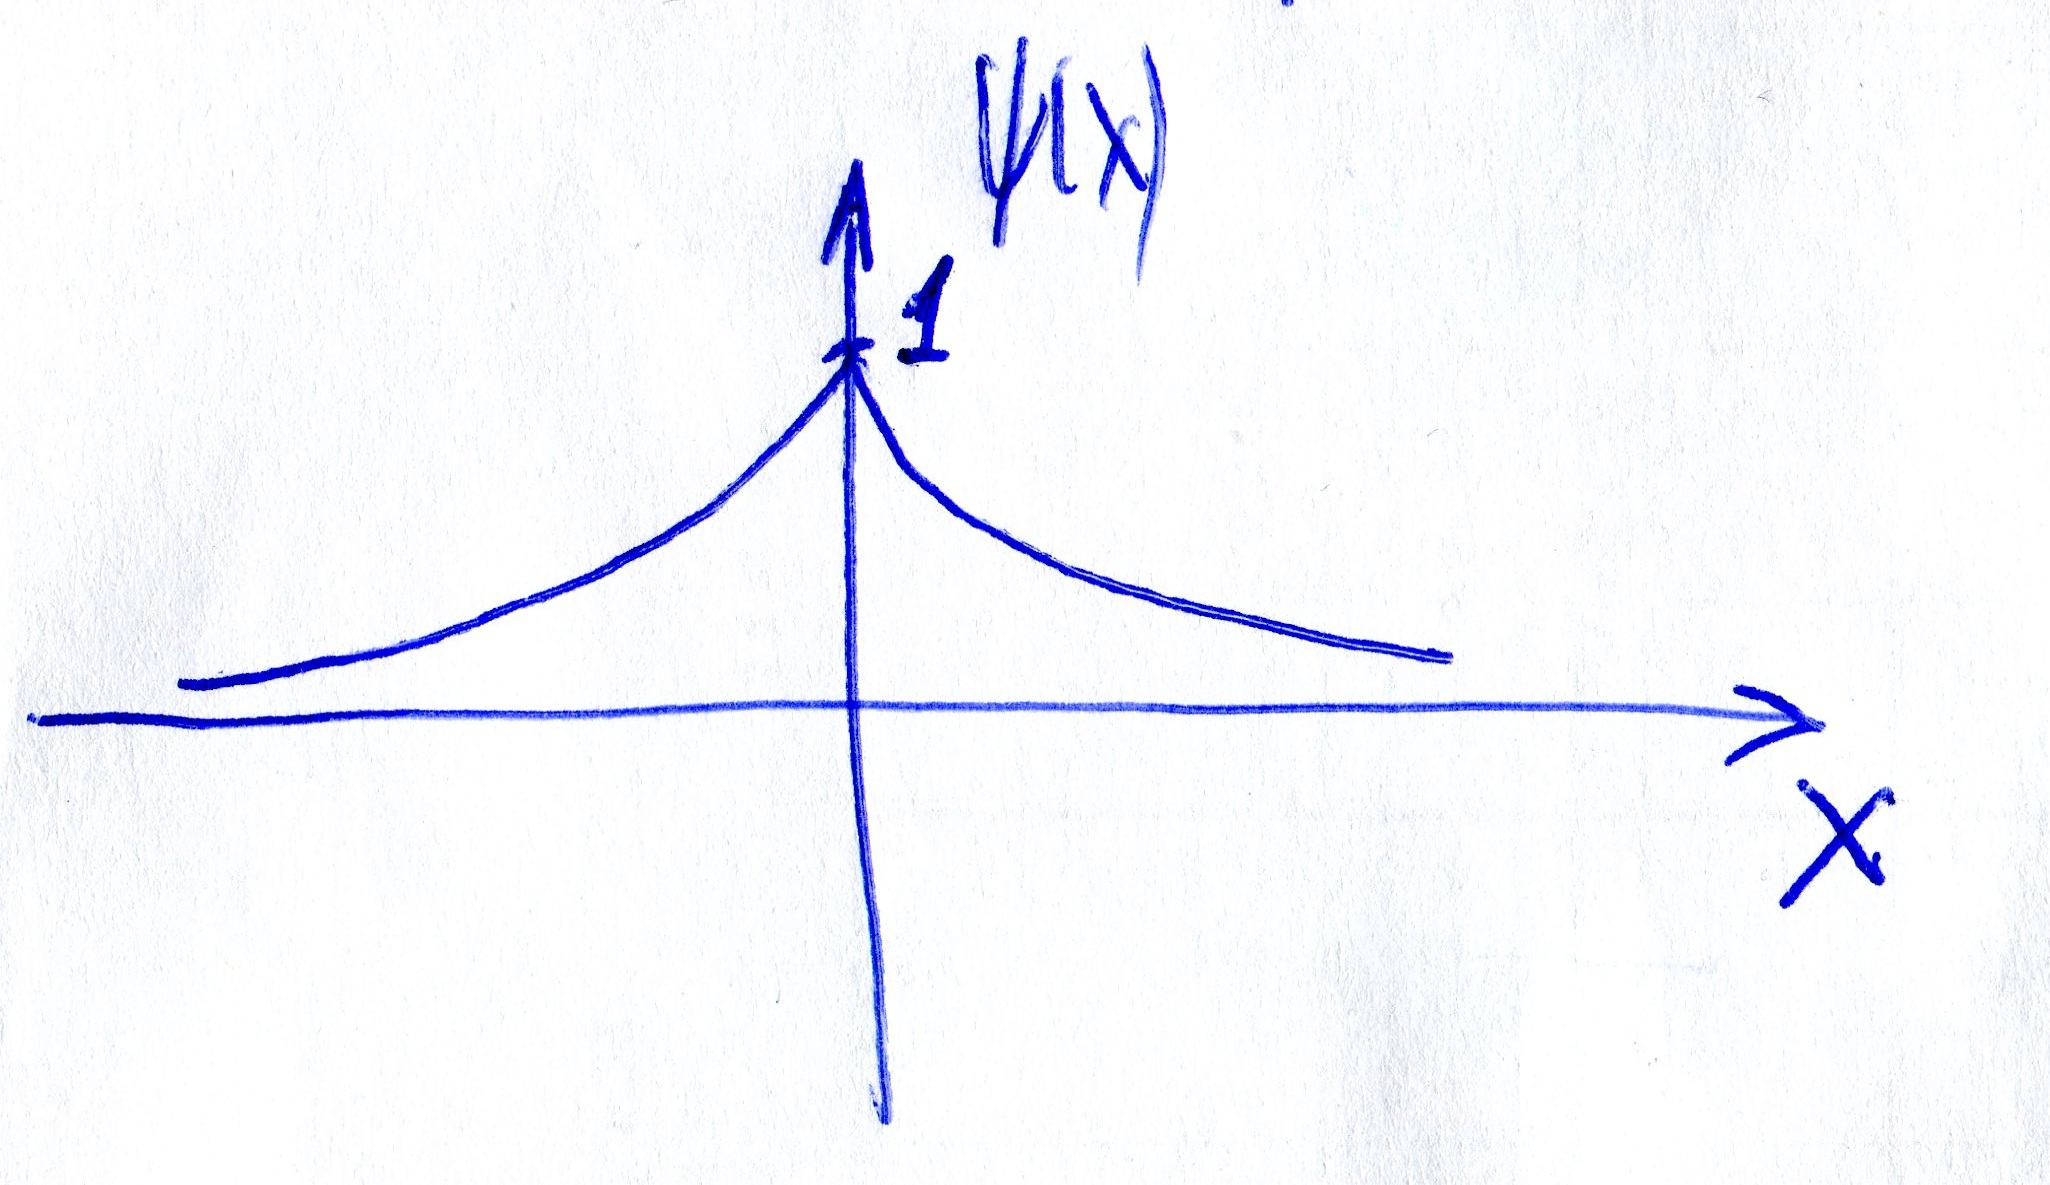
\includegraphics[width=\linewidth]{fig/fig73}
% \caption{}
% \vspace{-17pt}
% \end{wrapfigure}

$\Psi_0(x)=C\Psi(x)$ - нормировочная функция.

$$\int_{-\infty}^{+\infty}|\Psi_0(x)|dx = \int_{-\infty}^{+\infty}|\Psi(x)|^2C^2dx=1$$

$$\int_{-\infty}^{+\infty} e^{-2u|x|}dx=\int_{-\infty}^{0} e^{2ux}dx+\int_{0}^{+\infty} e^{-2ux}dx=\frac{1}{u}$$
$$\frac{C^2}{u}=1 \Longrightarrow C=\sqrt{u}$$
$$\Psi_0(x)=\sqrt{u}\exp{-u|x|}$$
$$\Psi(p)=\frac{1}{\sqrt{2\pi \hbar}}\int_{-\infty}^{+\infty} \Psi_0(x) e^{\frac{-ipx}{\hbar}}dx=\frac{\sqrt{u}}{\sqrt{2\pi \hbar}}\int_{-\infty}^{+\infty} e^{-u|x|} e^{\frac{-ipx}{\hbar}}dx=\sqrt{\frac{u}{2\pi \hbar}}\int_{-\infty}^{+\infty} e^{-(u|x|+\frac{ipx}{\hbar})}dx$$

Когда х>0
$$\int_{0}^{+\infty} e^{-(ux+\frac{-ipx}{\hbar})}dx=\int_{0}^{+\infty} e^{-x(u+\frac{ip}{\hbar})}dx=-\frac{1}{u+\frac{ip}{\hbar}}e^{-x(u+\frac{ip}{\hbar})} \bigg|_0^{+\infty}=\frac{\hbar}{\hbar u+ip}$$

Когда х<0
$$\int_{-\infty}^{0} e^{-(-ux+\frac{-ipx}{\hbar})}dx=\int_{-\infty}^{0} e^{-x(-u+\frac{ip}{\hbar})}dx=-\frac{1}{-u+\frac{ip}{\hbar}}e^{-x(-u+\frac{ip}{\hbar})} \bigg|_{-\infty}^0=-\frac{\hbar}{-\hbar u+ip}$$

$$\frac{\hbar}{\hbar u+ip}-\frac{\hbar}{-\hbar u+ip}=...=\frac{2\hbar ^2u}{p^2+\hbar ^2u^2}$$


$$\Psi(p)=\sqrt{\frac{u}{2\pi \hbar}} \cdot \frac{2\hbar ^2u}{p^2+\hbar ^2u^2}$$

% \begin{wrapfigure}{l}{0.3\linewidth}
% 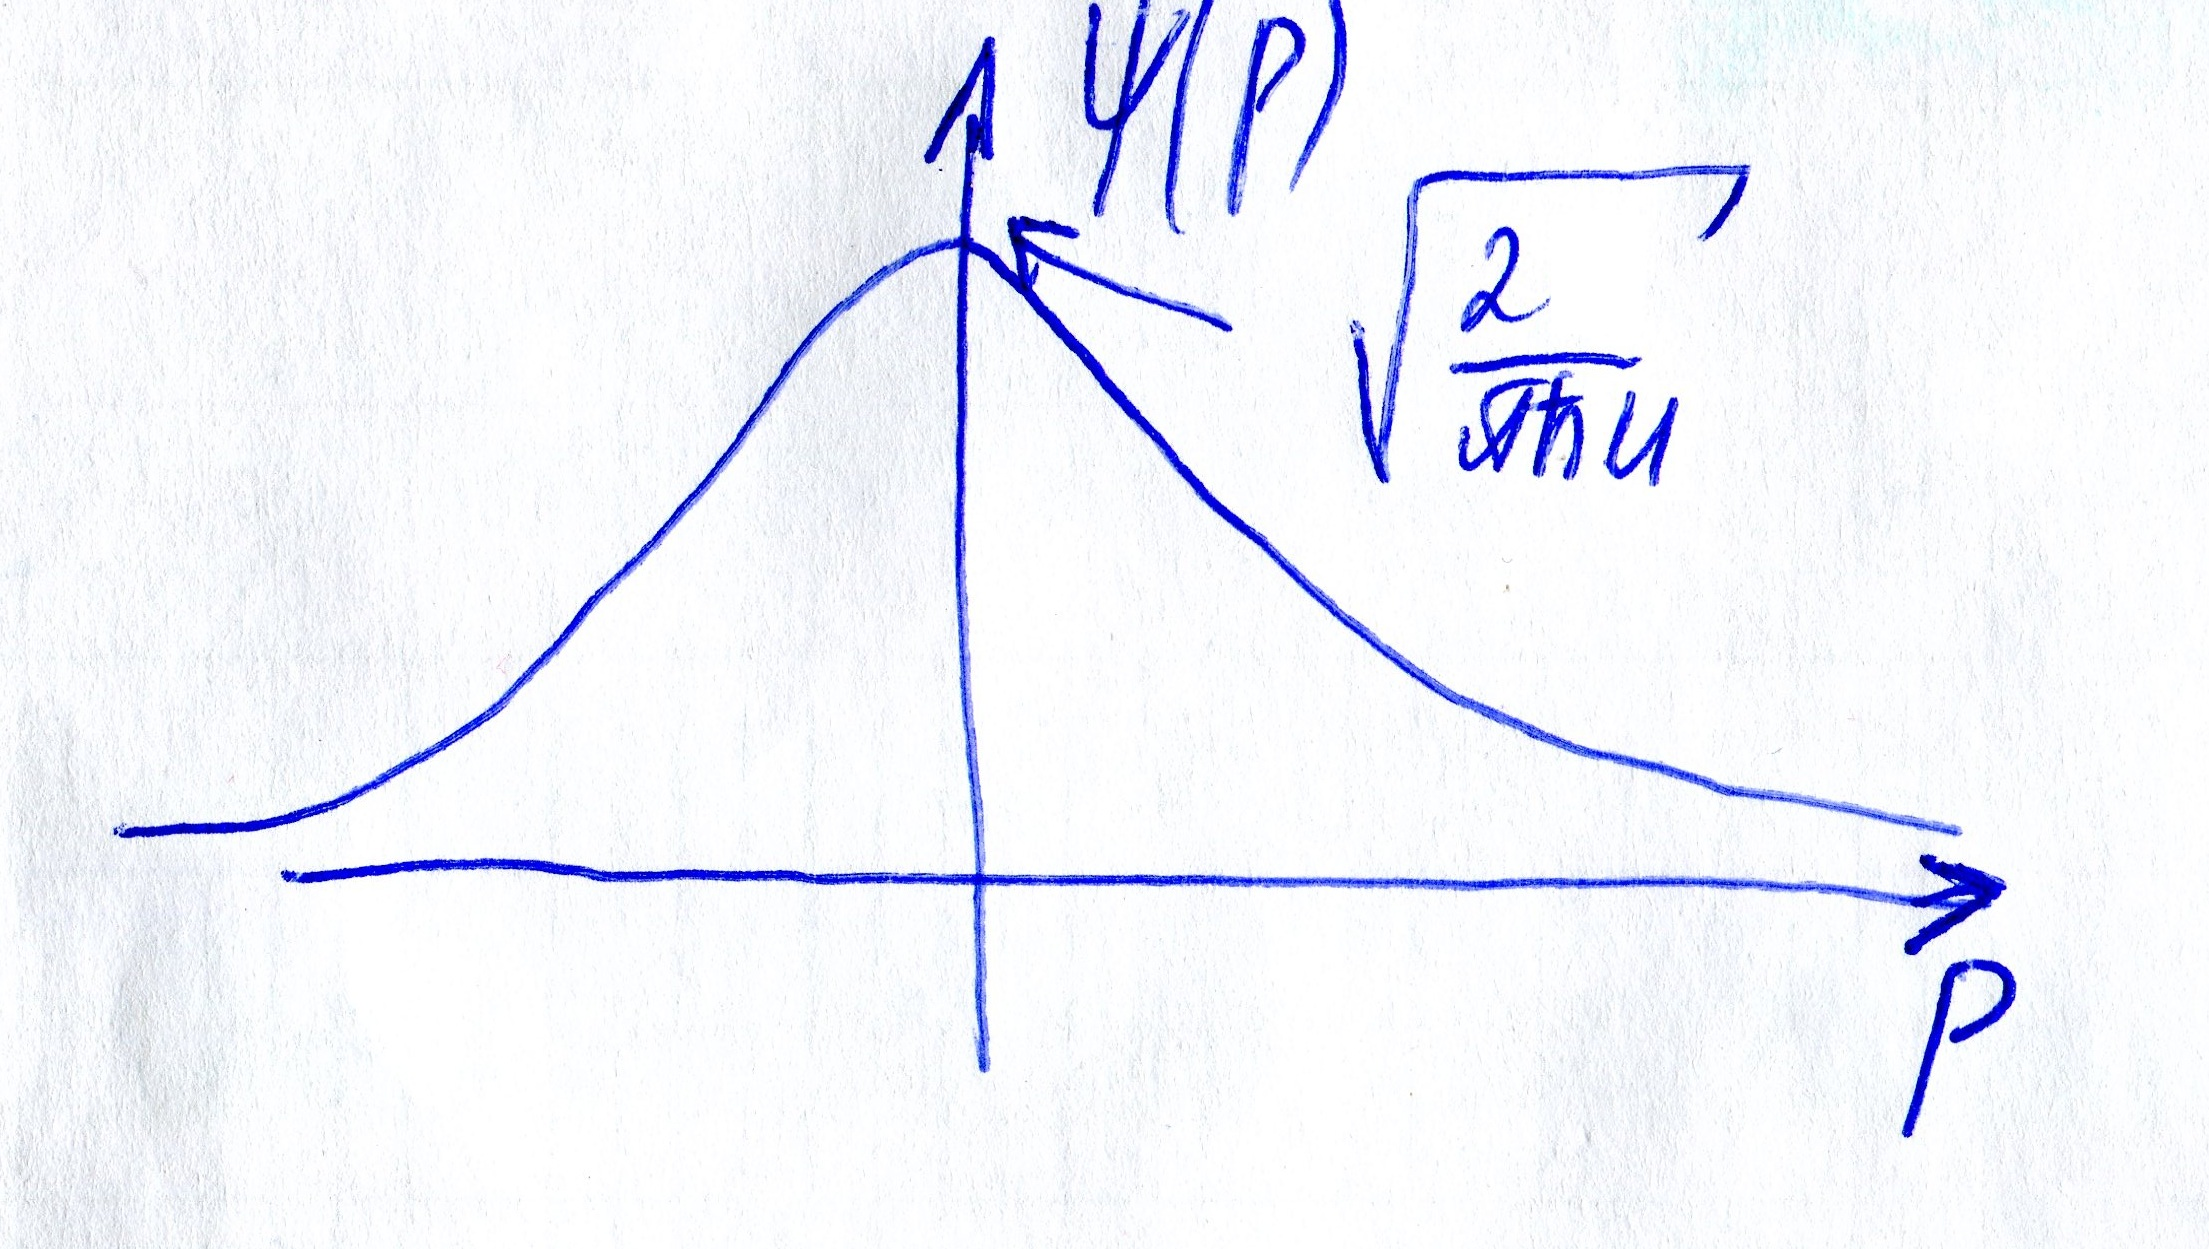
\includegraphics[width=\linewidth]{fig/fig731}
% \caption{}
% \vspace{-17pt}
% \end{wrapfigure}

 Ширина находится на уровне половины от максимума.
 $$\Psi(p=0)=\sqrt{\frac{2}{u\pi \hbar}}$$

 $$\Psi(p)=\sqrt{\frac{u}{2\pi \hbar}} \cdot \frac{2\hbar ^2u}{(1+\frac{p^2}{\hbar ^2u^2})\hbar ^2u^2}=\sqrt{\frac{1}{2\pi \hbar u}} \cdot \frac{2}{(1+\frac{p^2}{\hbar ^2u^2})}=\sqrt{\frac{2}{u\pi \hbar}} \cdot \frac{1}{(1+\frac{p^2}{\hbar ^2u^2})}=\Psi(p=0)\cdot \frac{1}{(1+\frac{p^2}{\hbar ^2u^2})}$$

 $$\Psi(p^*)=\frac{\Psi(p=0)}{2}$$
 $$\frac{1}{(1+\frac{p^{*2}}{\hbar ^2u^2})}=\frac12 \Longrightarrow p^*=\pm \hbar u $$ 
 $$\Delta p=2\hbar u$$

Найдем $\Delta x$ на уровне $e^{-1}$

$$\Psi(x^*)=\frac{\Psi(p=0)}{e} \Longrightarrow \exp{-u|x^*|}=\exp{-1} \Longrightarrow x^*=\pm \frac{1}{u}$$
 $$\Delta x=\frac{2}{u}$$
 $$\Delta x \cdot \Delta p= 4\hbar$$
 Соотношение неопределенностей позволяет проверить правильность решения. Произведение должно быть равно $\hbar$ с точностью до числового множителя.
\subsection{Билет 8}
%!TEX root = ../quantum.tex
\subsubsection{\textcolor{red} {Оператор импульса. Аналогия с классической механикой. Коммутатор с
координатой.} }
\subsubsection{Напишите разложение единичного оператора по собственным векторам к.л. оператора.}


Пусть есть некий оператор $\widehat{A}$.
$$\widehat{A}\ket{\psi_n} = a_n \ket{\psi_n},$$
где $\ket{\psi_n}$ - собственный вектор оператора.

В абстрактных обозначениях: $\ket{\psi_n} = \ket{n}$. Тогда
$$\widehat{1}=\sum_n C_n \ket{n}$$
Умножим скалярно на $\bra{\psi_m} = \bra{m}$
$$\bra{m} \widehat{1}=\sum_n \bra{m} C_n \ket{n}$$
Но если $m\neq n$, то $\ket{\psi_n}$ и $\ket{\psi_m}$ ортогональны. Следовательно, сумма отлична от нуля только при $m=n$ 
$$\bra{n} \widehat{1}=C_n, \bra{m}\widehat{1}=\bra{n}$$
$$\widehat{1}=\sum_n \ket{n} \bra{n}$$

\subsubsection{Нахождения волновой функции по данным одного из представлений}

Найдите $\Psi(p)$ по данным $\Psi(x)$. Найдите связь ширины в $x$ и $p$ представлениях. $\Psi(x)=\frac{1}{x^2+a^2}$.


$$\Psi(p)=\frac{1}{\sqrt{2\pi \hbar}} \int_{-\infty}^{+\infty} \Psi(x) e^{\frac{-ipx}{\hbar}}dx$$

1) $Im z>0, \lambda >0$. Используя лемму Жордана:
$$\int_{-\infty}^{+\infty} \frac{1}{x^2+a^2} e^{\frac{-ipx}{\hbar}}dx=2\pi i \sum_{k=1}^n res [R(z)\exp{i \lambda z}],$$
где $R(z)=\frac{1}{z^2+a^2}, \lambda=-\frac{p}{\hbar}$ 

Найдем особые точки 
$$R(z)= \frac{1}{z^2+a^2} = \frac{1}{(z+ia)(z-ia)}$$
$$z_0=\pm ia$$
Особе точки - полюса первого порядка. Внутри контура $L_1$ одна особая точка $z_0=ia$. Для полюса первого порядка

\begin{wrapfigure}{l}{0.3\linewidth}
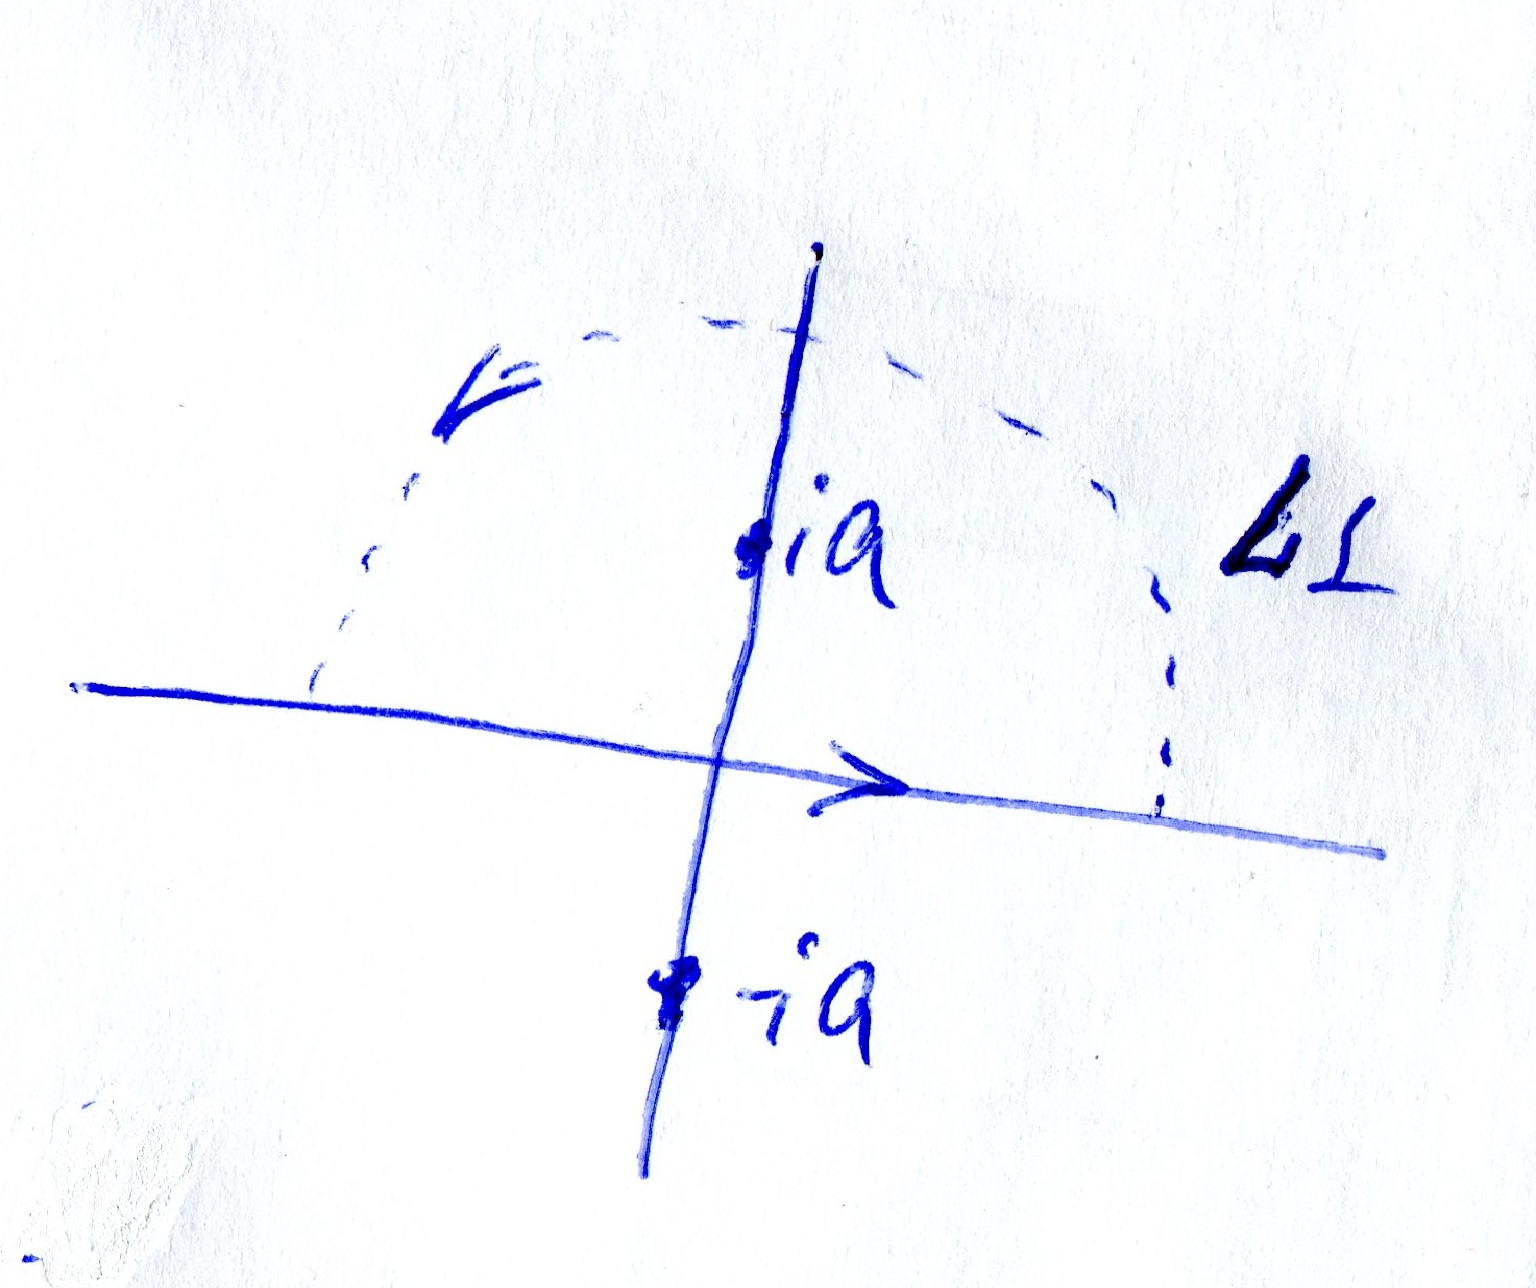
\includegraphics[width=\linewidth]{fig/fig83}
\caption{}
\vspace{-17pt}
\end{wrapfigure}

$$res f(z) = \frac{\varphi(z_0)}{\psi^{'}(z_0)},$$
где $f(z)=R(z)\exp{i \lambda z}$, $z_0$-особая точка, $\varphi(z)=\frac{\exp{i \lambda z}}{z+ia}, \psi(z)=z-ia, \psi^{'}(z)=1$.
$$res f(ia) = \frac{e^{i \lambda i a}}{2ia}$$
$$\int_{-\infty}^{+\infty} \frac{1}{x^2+a^2} e^{\frac{-ipx}{\hbar}}dx=\frac{2\pi e^{\frac{ap}{\hbar}}}{2ia}=\frac{\pi}{a} e^{\frac{ap}{\hbar}}, p<0$$

1) $Im z<0, \lambda <0, p>0$.
$$\int_{-\infty}^{+\infty} \frac{1}{x^2+a^2} e^{\frac{-ipx}{\hbar}}dx=-2\pi i \sum_{k=1}^n res [R(z)\exp{i \lambda z}],$$
Внутри контура $L_2$ одна особая точка $z_0=-ia$

\begin{wrapfigure}{l}{0.3\linewidth}
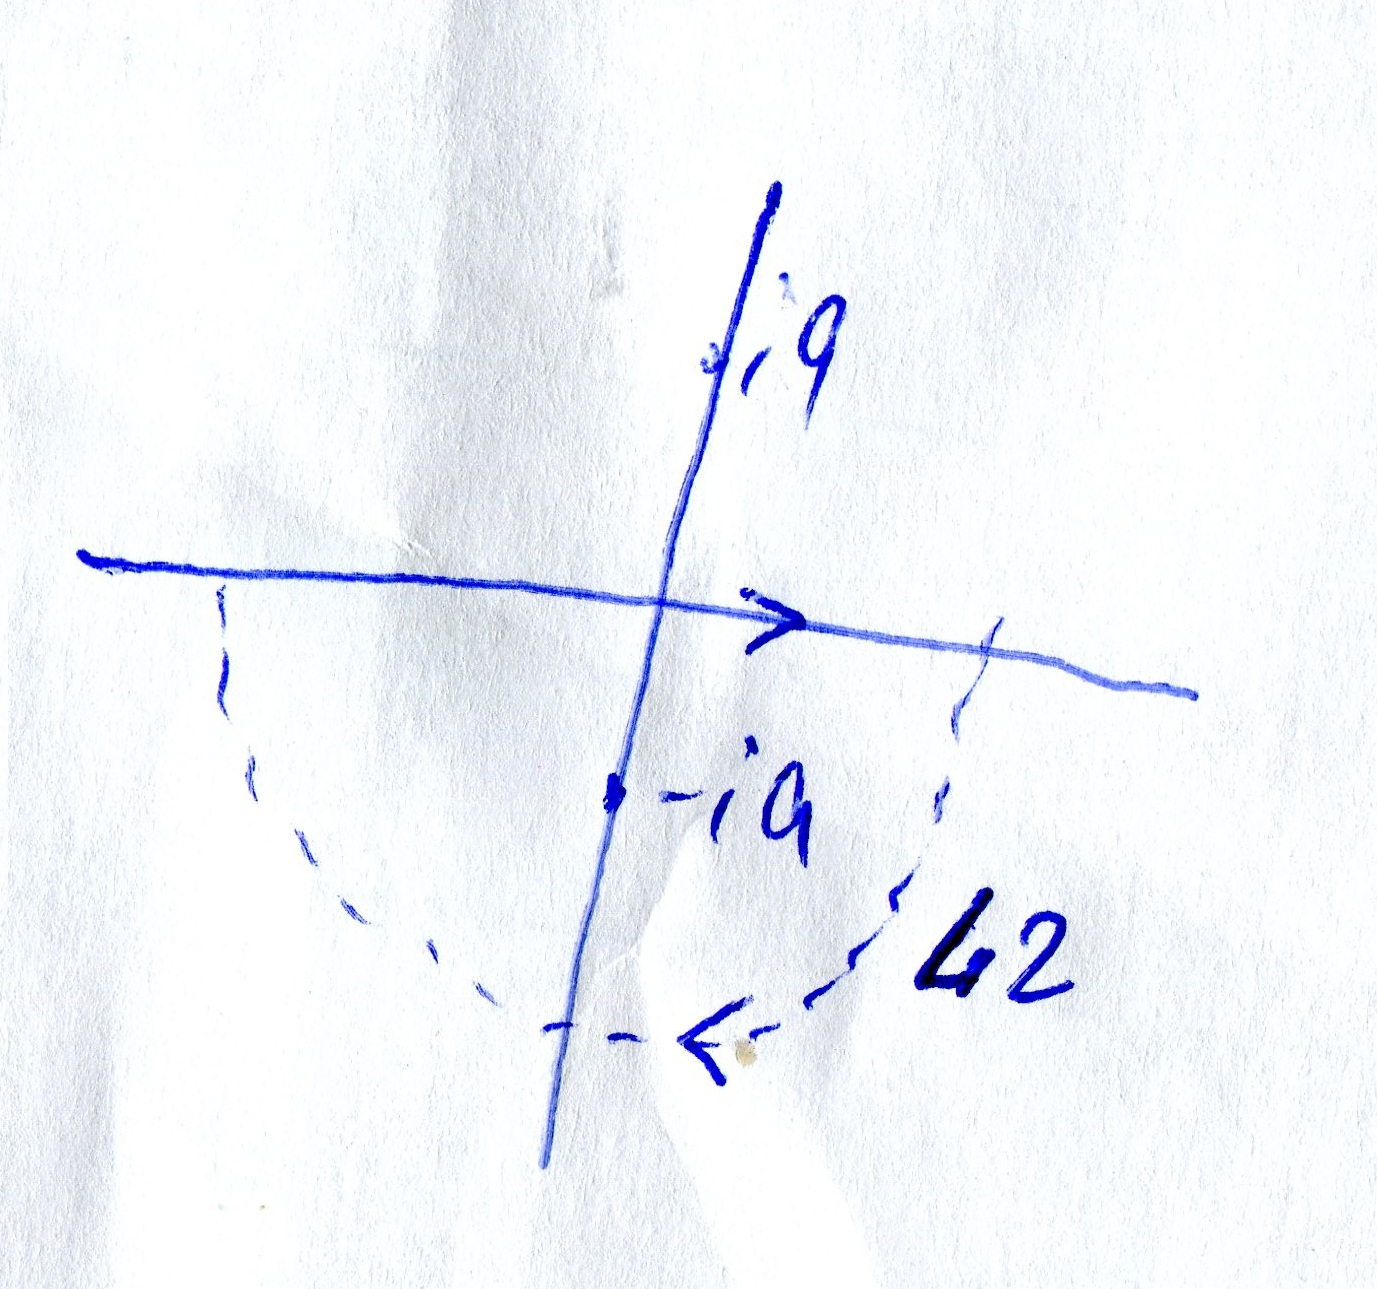
\includegraphics[width=\linewidth]{fig/fig831}
\caption{}
\vspace{-17pt}
\end{wrapfigure}

$res f(z) = \frac{\varphi(z_0)}{\psi^{'}(z_0)}, \varphi(z)=\frac{\exp{i \lambda z}}{z-ia}, \psi(z)=z+ia, \psi^{'}(z)=1$.
$$res f(-ia) = \frac{e^{\lambda a}}{-2ia}$$
$$\int_{-\infty}^{+\infty} \frac{1}{x^2+a^2} e^{\frac{-ipx}{\hbar}}dx=\frac{-2\pi i e^{a\lambda}}{-2ia}=\frac{\pi}{a} e^{a\lambda}=\frac{\pi}{a} e^{\frac{-ap}{\hbar}}, p>0$$
$$\int_{-\infty}^{+\infty} \frac{1}{x^2+a^2} e^{\frac{-ipx}{\hbar}}dx=\frac{\pi}{a} e^{\frac{-a|p|}{\hbar}}$$
$$\Psi(p)=\frac{\pi}{a\sqrt{2\pi \hbar}}e^{\frac{-a|p|}{\hbar}}$$

Эта функция еще не нормирована. При нормировке амплитуда не важна.
 $$\Psi_0(p)=C e^{\frac{-a|p|}{\hbar}}$$
 $$\int_{-\infty}^{+\infty} |\Psi_0|^2 dp=C^2 \int_{-\infty}^{+\infty}e^{\frac{-a|p|}{\hbar}} dp= 2C^2 \int_{0}^{+\infty}e^{\frac{-ap}{\hbar}}dp=\frac{C^2\hbar}{a}$$
 Нормировка $\frac{C^2\hbar}{a}=1 \Longrightarrow C=\sqrt{\frac{a}{\hbar}}$ 
 $$\Psi_0(p)=\sqrt{\frac{a}{\hbar}} e^{\frac{-a|p|}{\hbar}}$$
 Найдем $\Delta p$ на уровне $e^{-1}$.
 $$-\frac{a|p^*|}{\hbar}=-1 \Longrightarrow p^*=\pm \frac{\hbar}{a} \Longrightarrow \Delta p=\frac{2\hbar}{a}$$
$\Delta x$ находится на уровне половины от максимума.
$$\Psi(x^*)=\frac{1}{2a^2}$$
$$\frac{1}{2a^2}=\frac{1}{x^{*2}+a^2} \Longrightarrow x^*=\pm a \Longrightarrow \Delta x=2a$$
$$\Delta x \cdot \Delta p= 4\hbar$$
 Соотношение неопределенностей позволяет проверить правильность решения. Произведение должно быть равно $\hbar$ с точностью до числового множителя.


\subsection{Билет 9}
%!TEX root = ../quantum.tex
\subsubsection{Вопрос 1}
Разложите $\delta(x)$  по собственным функциям оператора импульса.

$\Psi(x)=\frac{1}{\sqrt{2\pi \hbar}}e^{\frac{i\pi x}{\hbar}}$ - нормированная собственная функция оператора импульса. Разложим по собственным функциям оператора импульса:

$$\delta(x) = \frac{1}{\sqrt{2\pi \hbar}}\int_{-\infty}^{+\infty} C(p) e^{\frac{i\pi x}{\hbar}} dp$$
$$C(p)=\bra{\Psi^*} \ket{\delta(x)}=\Psi^*(0)$$
$$\Psi^*(0)=\frac{1}{\sqrt{2\pi \hbar}}$$
$$\delta(x) = \frac{1}{\sqrt{2\pi \hbar}}\int_{-\infty}^{+\infty} \frac{1}{\sqrt{2\pi \hbar}} e^{\frac{i\pi x}{\hbar}} dp$$
$$\delta(x) = \frac{1}{2\pi \hbar}\int_{-\infty}^{+\infty} \ e^{\frac{i\pi x}{\hbar}} dp$$
\subsection{Билет 10}
%!TEX root = ../quantum.tex
\subsubsection{Преобразование Фурье как разложение по собственным функциям оператора импульса.}

$-i\hbar \frac{\partial{\Psi(x)}}{\partial x}=p_x \Psi(x)$ - операторное уравнение по собственным функциям импульса.

$-i\hbar \nabla$ - оператор импульса.

$$-i\hbar \dd \Psi(x)=p_x \Psi(x)\dd x$$
$$-i\hbar \ln(\Psi(x))=p_xx +C$$
$$\Psi(x)=\widetilde{C} e^{-\frac{p_xx}{i\hbar}}$$
Т.к. $\Psi(x)$ и $\widetilde{C} \Psi(x)$ описывают одно и то же состояние квантовой системы, отбросим константу. 

$\Psi(x)=e^{\frac{p_xx}{-i\hbar}}=e^{\frac{ip_xx}{\hbar}}$ - волна Де Бройля, собственная функция оператора импульса. Фурье-образ:
$$\Psi(x)=\int \Psi(p) e^{\frac{ip_xx}{\hbar}} dx$$
 С учетом нормировки в одномерном случае:
 $$\Psi(x)=\frac{1}{\sqrt{2\pi \hbar}}\int \Psi(p) e^{\frac{ip_xx}{\hbar}} dx$$

\subsubsection{Докажите, что нормировка сохраняется при замене представления, если использовать нормированные собственные функции }

$$\infint \abs{\Psi(x)}^2 \dd{x} = \infint \abs{\Psi(p)}^2 \dd{p}$$
По теореме Парсиваля:
$$\infint g^*(x) f(x)=\infint G^*(p) F(p) \dd{p}, $$
где $G(p)=F[g(x)]$, $F(p)=F[f(x)]$.

Тогда

$$\infint \Psi(x)^*\Psi(x) \dd{x} = \infint \Psi(p)^*\Psi(p) \dd{p} $$
$$\infint \abs{\Psi(x)}^2 \dd{x} = \infint \abs{\Psi(p)}^2\dd{p}  $$
Что же, осталось только доказать теорему Парсиваля.

{\centering\textbf{Доказательство} \\}

\begin{flushleft}
	
Пусть:

$\phi_0=\phi_1(x)\phi_2(x)$

Известно что:

$\Phi_1(p)=F[\phi_1(x)]$

$\Phi_2(p)=F[\phi_2(x)]$

Найдём:
$\Phi_0(p)=F[\phi_1(x)\cdot\phi_2(x)]$

\end{flushleft}
% Ща снова буит мясо
\begin{gather*}
\Phi_0(p)=\frac{1}{\sqrt{2 \pi \hbar}} 
\infint \phi_1(x)\phi_2(x)\exp{-\frac{ipx}{\hbar}} \dd x =\\
\frac{1}{\sqrt{2 \pi \hbar}}
\infint \frac{1}{\sqrt{2 \pi \hbar}} 
\infint \Phi_1(p')\exp{+\frac{ip' x}{\hbar}}\dd{p'}\cdot \phi_2(x)\exp{-\frac{ipx}{\hbar}}\dd{x}=\\
\frac{1}{2\pi\hbar}
\infint \infint \Phi_1(p')
\exp{\frac{ix(p'-p)}{\hbar}}\dd{p'}
 \cdot\phi_2(x)\dd{x}=\\
\frac{1}{2\pi\hbar}
\infint\infint\phi_2(x)\exp{\frac{ix}{\hbar}(p'-p)}\dd{x}\cdot\Phi_1(p' )\dd{p'}=\\
\qty{\frac{1}{2\pi\hbar}\infint\phi_2(x)\exp{\frac{ix}{\hbar}(p'-p)}=\Phi_2(p-p')}=\\
\frac{1}{\sqrt{2\pi\hbar}}\infint \Phi_2(p-p')\Phi_1(p')\dd{p'}
\end{gather*}

Получили, что 
$$\Phi_0=\frac{1}{\sqrt{2\pi\hbar}}\infint \Phi_2(p-p')\Phi_1(p')\dd{p'}=
\frac{1}{\sqrt{2\pi\hbar}} \infint \phi_1(x)\phi_2(x) e^{-\frac{ipx}{\hbar}} \dd{x}$$

Пусть $p=0$, тогда 
$$\Phi_0(0)=\frac{1}{\sqrt{2\pi\hbar}} \infint \phi_1(x)\phi_2(x)\dd{x}$$
$$\infint \Phi_2(-p' )\Phi_1(p' )\dd{p'}= \infint \phi_1(x) \phi_2(x)\dd{x} $$
По свойству преобразования Фурье:
$$F[\phi^*(x)]=\Phi^*(-p) $$
Получаем:
$$\infint \Phi_2'^*(p)\Phi_1(p') \dd{p'} = \infint \phi_1 \phi^*_2(x) \dd{x} $$
Что и требовалось доказать. \qed

\subsubsection{\textcolor{red} {Выведите уравнения Гейзенберга для частицы в потенциале. Сформулируйте
условие сохранения физической величины. Когда сохраняется энергия? Импульс?} }
\subsection{Билет 11}
%!TEX root = ../quantum.tex
\subsubsection{Нахождения волновой функции по данным одного из представлений}


\subsection{Билет 12}
%!TEX root = ../quantum.tex
\subsubsection{Задача.Нахождения волновой функции по данным одного из представлений}

$$\Psi(x)= \exp{-U\abs{x-x'} +ivx  }$$
$\Psi_0(x)$-- нормированная функция $\Psi$. $\Psi_0(x)=c\Psi(x)$.
$$\infint \abs{\Psi_0(x)}^2 \dd{x}=1$$
\begin{gather*}
	c^2\infint \Psi(x)^*\cdot\Psi(x)\dd{x}=
	\\ \frac{c^2}{2U}\exp{2U(x-x')}\eval_{-\infty}^{x'}- 
	\frac{c^2}{2U}\exp{-2U(x-x')}
	\eval^{\infty}_{x'}
\end{gather*}
Проводя очевидные действия находим нормировочную постоянную $c=\sqrt{U}$

Тогда $\Psi_0(x)=\sqrt{U}\exp{-U\abs{x-x'}+ivx}$.

\begin{gather*}
\Psi(p)=\frac{1}{\sqrt{2\pi\hbar}}\infint \Psi_0(x)\cdot\exp{-\frac{px}{\hbar}} \dd{x}=\\
\sqrt\frac{U}{2 \pi \hbar } \infint \exp{-U\abs{x-x'}}\exp{-ivx}\exp{-\frac{ipx}{\hbar}} \dd{x}
\end{gather*}
Обозначим $\tilde{\Psi}(x)=\sqrt{U} \exp{-u\abs{x-x'}}$,
 тогда $\Psi_0(x)=\tilde{\Psi}(x)\cdot\exp{ivx}$

Преобразуем $\tilde{\Psi}(x)\longrightarrow \tilde{\Psi}(p)$ 
%сейчас будет охрененно большой gather
\begin{gather*}
	\tilde{\Psi}(p)=\frac{1}{\sqrt{2\pi\hbar}}\infint\tilde\Psi(x)\exp{-\frac{ipx}{\hbar}} \dd{x} =\sqrt{\frac{U}{2 \pi \hbar}} \infint \exp{-U\abs{x-x'}}\exp{-\frac{ipx}{\hbar}}\dd{x} =\\
	\sqrt{\frac{U}{2 \pi \hbar}} \left(
	\int\limits_{-\infty}^{x'} \exp{+U (x-x')}\exp{-\frac{ipx}{\hbar}}\dd{x} 
	+
	\int\limits^{\infty}_{x'} \exp{-U (x-x')}\exp{-\frac{ipx}{\hbar}}\dd{x}
	\right)\\=
	\sqrt{\frac{U}{2 \pi \hbar }}\exp{-\frac{ipx' }{\hbar}}
	\qty
	(\int\limits_{-\infty}^0 e^{Uy} e^{-\frac{ipy}{\hbar}}\dd y+
	\int\limits^{\infty}_0 e^{-Uy} e^{-\frac{ipy}{\hbar}}\dd y
	 )
	 =\\
	 \sqrt{\frac{U}{2 \pi \hbar}} \exp{-\frac{ipx' }{\hbar}} 
	 \qty(\frac{1}{U-\frac{ip}{\hbar}} + \frac{1}{U+\frac{ip}{\hbar}})=\\
	 \frac{2}{U\qty(1+\frac{p^2}{U^2\hbar^2})}\sqrt{\frac{U}{2 \pi \hbar}} \exp{-\frac{ipx'}{\hbar}}=\sqrt{2}{U \pi \hbar} \frac{1}{1+\frac{p^2}{U^2\hbar^2}}\exp{-\frac{ipx' }{\hbar}}=\tilde {\Psi}(x). 
\end{gather*}
Напомним, что $\Psi_0(x)=\tilde\Psi(x)e^{ivx}$. Согласно замечанию 2:
	 $$\Psi(p)=\tilde{\Psi}(p-\hbar v)$$
И окончательный ответ:
	 $$\Psi(p)=\sqrt{\frac{2}{U\pi\hbar}}\cdot\frac{1}{1+\frac{(p-\hbar v)^2}{U^2\hbar^2}}\exp{-\frac{i(p-\hbar v)x' }{\hbar}} $$
\subsubsection{\textcolor{red} {Напишите решение УШ для свободного движения.} }

\subsubsection{{Выразить среднее в произвольном представлении} }

Тоже самое, что и в билете 4, только следует сказать, что волновая функция может быть любой.
\subsection{Билет 13}
%!TEX root = ../quantum.tex
\subsubsection{Нахождения волновой функции по данным одного из представлений}

$$\Psi(x)=\exp \qty{-\frac{(x-x')^2}{4b^2}+iUx} $$
В этом билете функция нормироваться не будет, так как автору стало лень, а на самом деле её и не просят. К тому же, на полу ширину нормировка не влияет.

$$\Psi(p)=\frac{1}{\sqrt{2\pi\hbar} } \infint \Psi(x) \exp{-\frac{ipx}{\hbar}}\dd{x} $$
Иначе говоря, $\Psi(p)=F[\Psi(x)]$.

По свойствам преобразования Фурье:  
\begin{enumerate}
	\item $\Psi_1(p-U\hbar)= F[\Psi_1(x)e^{iUx}]$ $\Psi_1(x)=\exp \qty{-\frac{(x-x')^2}{4b^2}}$
	\item $\Psi_2(p)\exp{-\frac{ipx'}{\hbar}}=F[\Psi_2(x-x')]$, где 
	$\Psi_2(x)=\exp \qty{-\frac{(x)^2}{4b^2}}$
\end{enumerate}

Найдем преобразование Фурье $\Psi_2(x)$ по определению.

\begin{gather*}
\Psi_2(p)=\frac{1}{\sqrt{2\pi\hbar}}\infint \exp{-\frac{x^2}{4b^2}+\frac{-ipx}{\hbar}}=\\
\frac{1}{\sqrt{2\pi\hbar}}\infint \exp{-\qty(\frac{x}{2b}+\frac{ipb}{\hbar})^2+
\qty(\frac{ipb}{\hbar})^2}\dd{x}= \\
\frac{1}{\sqrt{2\pi\hbar}}\exp{-\frac{p^2b^2}{\hbar^2}} 
\infint \exp{-\qty(\frac{x}{2b}+\frac{ipb}{\hbar})^2} \dd{x}=\\
\frac{2b}{\sqrt{2\pi\hbar}}\exp{-\frac{p^2b^2}{\hbar^2}} 
\infint \exp{-y^2}\dd{y}=\frac{2b\sqrt\pi}{\sqrt{2\pi b}}\exp{-\frac{p^2b^2}{\hbar^2}}=\\ 
\sqrt{\frac{2}{\hbar}}b\exp{-\frac{p^2b^2}{\hbar^2}}
\end{gather*}

Получим, что $\Psi_2(p)=\sqrt{\frac{2}{\hbar}}b\exp{-\frac{p^2b^2}{\hbar^2}}$.

$$\Psi_2(p)=F[\exp{-\frac{x^2}{4b^2}}]$$

Согласно свойству (2):
$$\sqrt{\frac{2}{\hbar}}b\exp{-\frac{p^2b^2}{\hbar^2}}\exp{-\frac{px'}{\hbar}}=
F[\Psi_2(x-x')]=F\qty[ \exp{-\frac{(x-x')^2}{4b^2}} ] = F[\Psi_1(x)]$$
Согласно свойству (1):
\begin{gather*}
\sqrt{\frac{2}{\hbar}}b\exp{-\frac{(p-U\hbar)^2b^2}{\hbar^2}}\exp{-\frac{i(p-U\hbar)x'}{\hbar}}=\\
 F\qty[\exp{-\frac{(x-x')^2}{4b^2}}+iUx]=F[\Psi(x)]
\end{gather*}
Что и требовалось найти.

\begin{equation}
	\Psi(p)=\sqrt{\frac{2}{\hbar}}b\exp{-\frac{(p-U\hbar)^2b^2}{\hbar^2}-\frac{i(p-U\hbar)x'}{\hbar} }
\end{equation}

Теперь найдем $\Delta p$. Она в $\Psi(p)$ такая же, как в $\Psi_2(p)$. Ищем полуширину на уровне $\frac{1}{e}$. Тогда
$$\Delta p=\frac{2\hbar}{b}$$
Найдем $\Delta x$на уровне $\frac1e$, при этом отбрасывая фазу.

\begin{gather*}
	-\frac{(x-x')^2}{4b^2}=-1 \\
	x_1=2b+x'\\
	x_2=x'-2b\\
	\Delta x= x_2-x_1=4b
\end{gather*}

$$\Delta x\cdot \Delta p=\frac{4b\cdot2\hbar}{b}=8\hbar  $$

\subsubsection{\textcolor{red} {На примере конкретного пакета продемонстрируйте соотношение неопределенности. Операторы как матрицы. Непрерывные и дискретные индексы.} }


\subsubsection{\textcolor{red} {Представления операторов умножения и дифференцирования как матриц.} }
\subsection{Билет 14}
%!TEX root = ../quantum.tex
\subsubsection{Амплитуда вероятности. Принцип суперпозиции. Сложение амплитуд. Мысленный эксперимент с двумя щелями}

Предположим, что есть два состояния квантовой системы $\Psi_1$ и $\Psi_2$.
Тогда, по принципу суперпозиции существует состояние $\Psi_3=c_1\Psi_1+c_2\Psi_2$,где
$c_1$ и  $c_2$-- комплексно значные величины, называемые амплитудами вероятности. $\Psi_3$ принимает состояние №1 с вероятностью $|c_1^2|$ и состояние №2 с вероятностью $|c_2|^2$. То есть при сложении двух волновых функций мы не получаем чего-то третьего, а получаем либо состояние №1 с вероятностью $|c_1^2|$, либо №2 с вероятностью $|c_2^2|$.

Одним из наблюдаемых следствий является прохождение электрона через две близко расположенные щели. Если две щели открыты одновременно, то на экране наблюдается интерференционная картина. Это объясняется тем, что электрон находится в суперпозиции состояний.
\begin{equation}
	\Psi(\vec{r},t)=\qty[\Psi_1(\vec{r})+\Psi_2(\vec{r})]\cdot\exp\qty(-\frac{iEt}{\hbar})
\end{equation}
Плотность вероятности нахождения электрона вблизи точки $(\vec{r},t)$ равна:
\begin{gather*}
	|\Psi(\vec{r},t)|^2=|\Psi_1(\vec{r})+\Psi_2(\vec{r})|^2=|\Psi_1(\vec{r},t)|^2+
	|\Psi_2(\vec{r},t)|^2+\qty(\Psi_1^*\Psi_2+\Psi_1\Psi_2^*)=\\
	|\Psi_2(\vec{r},t)|^2+|\Psi_1(\vec{r},t)|^2+2|\Psi_1|\cdot|\Psi_2|\cos(\phi_1-\phi_2)
\end{gather*}

Последнее слагаемое -- интерференционный член. Каждый электрон интерферирует сам  с собой, так как он вошел частично в каждую волну и невозможно точно сказать через какую из щелей он проходит.

\subsubsection{\textcolor{red} {Сформулируйте, что такое дискретный и непрерывный спектры. Каковы волновые
функции, как они нормируются.} }

\subsubsection{\textcolor{red} {Запишите общее решение нестационарного уравнения Шредингера с помощью
разложения по стационарным состояниям} }

\subsection{Билет 15}
%!TEX root = ../quantum.tex
\subsubsection{\textcolor{red} {Обозначения Дирака для векторов, волновых функций, операторов и матриц} }

\subsubsection{\textcolor{red} {Стационарные состояния. Энергетическое представление. Различные представления операторов. }}

\subsubsection{\textcolor{red} {Докажите, что собственные значения эрмитового оператора действительны.} }


\subsection{Билет 16}
%!TEX root = ../quantum.tex
\subsubsection{От каких переменных может зависеть волновая функция. Полный набор.}



Волновая функция должна полным образом описывать систему, а изменение волновой функции от времени полностью описывает эволюцию квантово-механической системы (Уравнение Шредингера). 

Существует несколько вариантов представления волновых функций (координатный, импульсный, энергетический и т.д). Соответственно, они могут быть описаны через разные переменные. 

Максимальная информация о системе (Полнота описания системы) определяет количество степеней свободы. Чтобы волновая функция полностью описывала систему, необходимо, чтобы количество ее переменных равнялось количеству степеней свободы. 

Переменными волновой функции могут быть собственные значения какого-то оператора. Одновременно являться переменными волновой функции могут быть лишь те величины, операторы которых коммутируют между собой. Соответственно, переменные волновой функции могут быть взяты даже из различных операторов, но главное, чтобы выполнялось условие коммутации. Сколько переменных необходимо для полного описания волновой функции? Количество переменных должно равняться количеству степеней свободы.

Дальше идет отсебятина: уверенности нет, но скорее всего это так. говорите на свой страх и риск. 

 Пример: для описания квантово-механической системы, состоящей из одного свободного электрона, на самом деле недостаточно знать координат или импульсов этой частицы, так как она обладает как минимум еще и спином., что дает ему еще как минимум одну степень свободы. Получаем, что у электрона степеней свободы как минимум 4 (x,y,z, проекции координат или импульсов +спин). 


\subsubsection{\textcolor{red} {Дайте определение среднего значения физической величины в каком-либо
состоянии.}}

\subsubsection{\textcolor{red} {Докажите теорему о полноте (разложении единицы)
$\delta(a-a')=\int\Psi_b^*(a)\Psi_b(a')\dd{b}$.
Запишите её в абстрактных Дираковских обозначениях. Какова должна быть
нормировка.} }
\subsection{Билет 17}
%!TEX root = ../quantum.tex
\subsubsection{Дайте определение сопряженного по Эрмиту оператора. Ответ сформулируйте в явной интегральной форме в $x$ представлении, в обозначениях Дирака и обычных абстрактных векторных обозначениях.}

% \newcommand{\definition}{\underset{def}{=}}
% \renewcommand{\big}{\displaystyle}



Сопряженным по Эрмиту оператором называется оператор, который и транспонирован, и сопряжен
$$A^+=A^{*T} $$
Сопряженным по Эрмиту оператором называется такой оператор, что 
$(\phi,A\Psi)\definition(A^+\phi,\Psi)$

\textbf{В интегральной форме:}

$$\big \int\phi^*(x)K(x,x')\Psi(x')\dd{x}\dd{x'}\definition\int N^*(x,x')\phi(x')\dd{x'}\Psi(x)\dd{x}=*$$
Обозначим ядро оператора $A^+$ как $N(x,x')$. Тогда $A^+\phi=\int N(x,x)'\phi(x')\dd{x'}$

$$\big *=\int N^*(x',x)\phi^*(x)\dd{x}\Psi(x')\dd{x'}$$

Тогда $\big N^*(x',x)=K(x,x')$

\textbf{В обозначениях Дирака}:
$$\ket{\Psi}=\hat{A}\ket{x}$$

Тогда эрмитово сопряжение:
$$\bra{\Psi}\definition\bra{x}\hat{A}^+$$

\textbf{В абстрактных векторных обозначениях:}

$$\ket{\Psi}^T=\ket{\Psi}^*, ~~ \text{но} (T*)=+$$

$$\ket{\Psi}^{T*}=\ket{\Psi}^{**} $$

Значит, что
$$\ket{\Psi}^+\definition \bra{\Psi} $$

\subsection{Билет 18}
%!TEX root = ../quantum.tex
\subsubsection{Докажите, что если операторы коммутируют, то они имеют общие собственные
функции.}




$$\hat{M}\hat{F}-\hat{F}\hat{M}=0$$
Пусть $\Psi_n$ образуют полную систему собственных функций оператор $\hat{M}$, то есть
$\hat{M}\Psi_n=M_n\Psi_n$.

Подействуем оператором $\hat{F}$

$$\hat{M}\hat{F}=\hat{F}\hat{M}$$
$$\hat{M}\hat{F}\Psi_n=\hat{F}\hat{M}\Psi_n=\hat{F}M_n\Psi_m=M_n\hat{F}\Psi_n $$
$$\hat{M}(\hat{F}\Psi_n)=M_n(\hat{F}\Psi_n), \hat{F\Psi_n}-\text{собственная функция оператора }\hat{M}$$
Следовательно $\hat{F}\Psi_n=\Psi_n$. $\hat{F}\Psi_n$ отличается от собственной функции только на константу, пусть $\const=F_n$

Тогда $\hat{F}\Psi_n=F_n\Psi_n.$

\subsubsection{Докажите, что оператор кинетической энергии эрмитов.}


$$\hat{T}=-\frac{\hbar^2}{2m}\nabla^2- \text{оператор кинетической энергии}$$
$$\hat{T_x}=-\frac{\hbar^2}{2m}\pdv[2]{x}$$
$$\big  \infint\phi^*\hat{T}\Psi \dd{x}=
\infint \hat{T}^+\phi^*\Psi \dd{x} - \text{определение эрмитовости}$$
\begin{gather*}  
\infint\phi^* \qty(\frac{-\hbar^2}{2m})
\qty(\pdv[2]{x}\Psi)\dd{x}=
\begin{bmatrix}
U=\phi^* & V=\pdv{\Psi}{x} \\
\dd{U}=\pdv{\phi^*}{x} & \dd{V}=\pdv[2]{x}\Psi\dd{x}
\end{bmatrix}=\\
\phi^*\pdv{\Psi}{x}\eval_{-\infty}^{\infty}\qty(\frac{\hbar^2}{2m})-
\qty(-\frac{\hbar^2}{2m})\infint
\pdv{\Psi}{x}\pdv{\phi^*}{x}\dd{x}
=*
\end{gather*}
В силу физических соображений первое слагаемое дает 0 (на бесконечности функция не может расти, а только спадать).

\begin{gather*}
*= -\qty(-\frac{\hbar^2}{2m})\infint
\pdv{\Psi}{x}\pdv{\phi^*}{x}\dd{x}= 
	\begin{bmatrix}
	U=\pdv{\phi^*}{x} & V=\Psi \\
	\dd{U}=\pdv[2]{\phi^*}{x}\dd{x} & \dd{V}=\pdv{\Psi}{x}\dd{x}
	\end{bmatrix}=\\
-\Psi\pdv{\phi^*}{x}\eval_{-\infty}^{\infty}\qty(-\frac{\hbar^2}{2m})+
\qty(-\frac{\hbar^2}{2m})\infint\pdv[2]{\phi^*}{x}\Psi\dd{x}\\=
\infint \qty(-\frac{\hbar^2}{2m}\pdv[2]{x})\Psi^*\Psi \dd{x}
\end{gather*}
Следовательно, $\hat{T}=\hat{T}^+$. Значит оператор кинетической энергии эрмитов.


\subsection{Билет 19}
%!TEX root = ../quantum.tex
\subsubsection{Оператор импульса. Связь с оператором сдвига.}



Оператор сдвига:
$$\hat{T}f(x)=f(x+a) $$

Пусть сдвиг мал $\delta a$.
$$\hat{T_{\delta a}}f(x)=f(x+\delta a)$$

Разложим в ряд Тейлора:
$$f(x+\delta a)= f(x) + \pdv{f}{x} \delta a + \pdv[2]{f}{x} (\delta a)^2+\dots$$
Домножим на $-i\hbar$ и поделим на $-i\hbar$:
$$p_x=-i\hbar\pdv{x}$$
$$f(x+\delta a)=f(x)+\qty(-\frac{\delta a}{i \hbar})pf+\qty(-\frac{\delta a}{i \hbar})^2p^2f+\dots $$
Получаем:
$$\hat{T}f(x)=\exp\qty(-\frac{\delta a}{i \hbar} p)f(x) - \text{связь оператора сдвига и импульса}$$


\subsubsection{\textcolor{red} {Замена представления. Обозначения Дирака.} }


\subsubsection{\textcolor{red} {Запишите нестационарное уравнение Шредингера в энергетическом представлении.
Найдите его общее решение. Как выглядит оператор H
в энергетическом
представлении} }
\subsection{Билет 20}
%!TEX root = ../quantum.tex
\subsubsection{Вопрос 1}

Какие значения может принимать некоторая физическая величина $A$ и с какой вероятность?

Физическая величина в квантовой механике есть наблюдаемая величина. Каждой наблюдаемой величине соответствует свой оператор. Существует операторное уравнение на собственные функции и собственные числа наблюдаемой $A$ .

$$\hat{A}\Psi=a\Psi$$
Решениями такого операторного уравнения являются пары $a_n,\Psi_n$. 

Если решения такого операторного уравнения счётны, то такой случай является дискретным. В противном случае, когда собственные числа не являются счётными, то такой случай называется непрерывным.

По постулатам квантовой механики: при измерении наблюдаемой величины получаются только собственные значения оператора $\hat{A}$. Если система наблюдается в состоянии $\Psi_n$,  то в результате её измерения получаем $a_n$ с вероятностью 1.

Если система находится в суперпозиции состояния $\Psi=c_1\Psi_1+c_2\Psi_2+\dots+C_k\Psi_k$, то при измерении системы вероятность получить $a_1$ есть $|c_1|^2$.
\subsection{Билет 21}
%!TEX root = ../quantum.tex
\subsubsection{Вопрос 1}

Вычислите оператор, сопряженный к произведению $AB$ . Сформулируйте условие эрмитовости произведения, если $A$ и $B$ эрмитовы.

Оператор $A^*$ называется сопряженным к оператору $A$ если $(\phi, Ax)=(A^*\phi,x).$

Вычислим оператор, сопряженный к произведению $AB$.

$$(\phi, ABx)= (A^*\phi,Bx)*=(B^*A^*\phi,x) $$
(*) к $A^*\phi$  относимся как к целому.

Тогда $(AB)^*=B^*A^*.$

Условие эрмитовости произведения, если $A$ и  $B$ эрмитовы:
произведение двух эрмитовых операторов является эрмитовым, если их коммутатор равен 0.

\subsubsection{Вопрос 3}
Докажите, что собственные функции эрмитового оператора, соответствующие разным собственным значениям, ортогональны.


\begin{equation}
\label{eq:3.1}
A\ket{\Psi_n}=a_n\ket{\Psi_n} 	
\end{equation}

Берем эрмитовое сопряжение:
\begin{equation}
	\label{eq:3.2}
\bra{\Psi_n}A^+=a_n^*\bra{\Psi_n} 
\end{equation}
Заменим в \eqref{eq:3.2} $n\rightarrow m$. Уравнение \eqref{eq:3.1} скалярно умножим на $\bra{\psi_m}$, \eqref{eq:3.2} умножим на $\ket{\Psi_n}$  и вычтем.

Получаем:
\begin{equation}
	\bra{\Psi_m}A\ket{\Psi_n}-\bra{\Psi_n}A^+\ket{\Psi_m}=(a_n-a^*_m)
	\braket{\Psi_m}{\Psi_n}=0
\end{equation}
n и m - разные, значит $a_n\neq a_m^*$. Следовательно $\braket{\Psi_m}{\Psi_n}=0$

$$\big \braket{\Psi_m}{\Psi_n}=\int \Psi_m^*(x)\Psi_n(x)\dd{x}=(\Psi_m,\Psi_n)=0 $$
\subsection{Билет 22}
%!TEX root = ../quantum.tex
\subsubsection{Покажите, что если два оператора, A и B имеют общие собственные функции, то
они коммутируют.}


\begin{gather*}
	\hat{B}\cdot\eval \hat{A}\Psi_n=a_n\Psi_n \\
	\hat{A}\cdot\eval \hat{B}\Psi_n=b_n\Psi_n
\end{gather*}
\begin{equation*}
\begin{cases}
	\hat{B}\hat{A}\Psi_n=a_n\hat{B}\Psi_n \\
	\hat{A}\hat{B}\Psi_n=b_n\hat{A}\Psi_n
\end{cases}
\end{equation*}

\begin{equation*}
\begin{cases}
	\hat{B}\hat{A}\Psi_n=a_nb_n\Psi_n \\
	\hat{A}\hat{B}\Psi_n=b_na_n\Psi_n \\
\end{cases}
\end{equation*}
Вычтем из первого уравнения второе:
\begin{equation*}
	(\hat{B}\hat{A}-\hat{A}\hat{B})\Psi=\sum\limits_n a_n (\hat{B}\hat{A}-\hat{A}\hat{B})\Psi_n=0
\end{equation*}
Следовательно $\hat{A}$  и $\hat{B}$ коммутируют.

\subsubsection{\textcolor{red}{Как выглядит оператор в своём собственном представлении. Как устроены волновые функции в этом представлении?}}

\subsubsection{\textcolor{red}{Напишите уравнение движения квантовой частицы в однородном поле $U=-Fx$ в импульсном представлении}}
\subsection{Замечание 1}
При нормировке функции $\Psi$ важна лишь ее форма, а не амплитуда, так как
существует лишь один вариант сделать единичную площадь у фигуры
заданной формы. Поэтому, при определении нормы амплитуда изначальной
функции $\Psi$ не важна, а важна лишь форма, следовательно, амплитуда
может быть произвольной и выбираться с точки зрения упрощения решения
задачи.
\subsection{Замечание 2}
$$\Psi_1=\Psi(x)e^{i \alpha x} $$
$$\Psi_1 = \frac{1}{\sqrt{2\pi\hbar}}\infint \Psi_1(x) e^{-\frac{ipx}{\hbar}} \dd x$$
\begin{gather}
\Psi_1(p)=\frac{1}{\sqrt{2\pi\hbar}}\infint \Psi(x) e^{i \alpha x} e^{-\frac{ipx}{\hbar}} \dd x =\\
\frac{1}{\sqrt{2\pi\hbar}}\infint \Psi(x) e^{-\frac{ix}{\hbar}(p-\hbar \alpha)}=\Psi(p-\hbar \alpha)
\end{gather}
\end{document}
